\documentclass[12pt, letterpaper]{article}
\usepackage{amsmath}
\usepackage{amssymb}
\usepackage{braket}
\usepackage{fancyhdr}
\usepackage{geometry}
\usepackage{graphicx}
\usepackage{listings}
\usepackage{mathtools}
\usepackage{physics}
\usepackage{titlesec}
\usepackage{tikz-feynman}
\usepackage{import}
\usepackage{xifthen}
\usepackage{pdfpages}
\usepackage{transparent}

\newcommand{\N}{\mathbb{N}}
\newcommand{\Z}{\mathbb{Z}}
\newcommand{\Q}{\mathbb{Q}}
\newcommand{\R}{\mathbb{R}}
\newcommand{\C}{\mathbb{C}}

\newcommand{\incfig}[2][1]{%
  \def\svgwidth{#1\columnwidth}
  \import{./figures/}{#2.pdf_tex}
}

\pdfsuppresswarningpagegroup=1

\geometry{a4paper, total={170mm,257mm}, left=20mm, top=20mm,}
\newcommand{\dbar}{\dd\hspace*{-0.18em}\bar{}\hspace*{0.1em}}

\usepackage[many]{tcolorbox}

\definecolor{backcolour}{rgb}{0.25,0.25,0.22}

\tcolorboxenvironment{lstlisting}{
  spartan,
  frame empty,
  boxsep=0mm,
  left=1mm,right=1mm,top=-1mm,bottom=-1mm,
  colback=backcolour,
}

\definecolor{codegreen}{rgb}{0.5,0.9,0.6}
\definecolor{codegray}{rgb}{0.5,0.5,0.5}
\definecolor{codepurple}{rgb}{0.58,0,0.82}
\definecolor{codebeige}{rgb}{0.90,0.80,0.55}

\lstdefinestyle{mystyle}{
    backgroundcolor=\color{backcolour},
    commentstyle=\color{gray},
    keywordstyle=\color{codebeige},
    numberstyle=\tiny\color{codegray},
    stringstyle=\color{codegreen},
    basicstyle=\ttfamily\footnotesize\color{white},
    breakatwhitespace=false,
    breaklines=true,
    captionpos=b,
    keepspaces=true,
    numbers=none,
    numbersep=5pt,
    showspaces=false,
    showstringspaces=false,
    showtabs=false,
    tabsize=2
}

\lstset{style=mystyle}

%\titleformat{\section}
%{\bfseries}
%{}
%{0em}
%{}
%
%\titleformat{\subsection}
%{\bfseries}
%{}
%{0em}
%{}

\author{Tom Rindell}
\title{}

\pagestyle{fancy}
\pagenumbering{gobble}

%\rhead{\textsc{HEADER}}
\lhead{\textsc{Tools of HPC}}
\rhead{\textsc{Final Project 2}}
%\lhead{\textsc{Tom Rindell\\014605789}}


\begin{document}
\begin{titlepage}
  \begin{center}
    \vspace*{5cm}
  \Huge{\bfseries Poisson's equation in two dimensions}\\
  \textsc{\LARGE Tools of High Performance Computing}\\
  \vfill
  \end{center}
  \begin{flushright}
  \textsc{\large Tom Rindell}\\
  \textsc{\large 014605789}\\
  \textsc{\large \today}\\
  \end{flushright}
\end{titlepage}

\section{Description}
The program presented here is used to solve a two-dimensional Poisson's equation on a unit square.
The solution is computed by the means of successive over relaxation (SOR) algorithm.
A brief overview of the used methods are given, explaining basic principles SOR. 
Following this, we discuss the motivation for parallelizing SOR, focusing on the potential improvements in speed and efficiency.

The program is parallelized to be run on multiple CPU cores for faster computation.
%This report presents the background and description of the SOR algorithm as well as the methods used for its parallelization.
The report details the design and implementation of the parallel algorithm, including the strategies used for dividing tasks among processors and ensuring synchronization. 
We also outline the specific parallelization techniques applied and the steps taken to optimize performance.

To evaluate the effectiveness of the algorithm, a series of tests are performed to compare its execution time and convergence behavior to that of the standard SOR algorithm. 
These tests are conducted on a personal laptop running 
%various computational setups to illustrate the scalability and efficiency improvements offered by parallelization.

\section{Background on SOR}
The problem of interest is the Poisson's equation on the unit square:
\begin{align*}
  \frac{\partial^2}{\partial x^2}f(x,y)
  +\frac{\partial^2}{\partial y^2}f(x,y)
  &=g(x,y),\qquad(x,y)\in[0,1]^2.
\end{align*}
The boundary conditions at $x,y\in \{0,1\}$ as well as the function $g(x,y)$ are known.
As the goal is to acquire numerical solutions to the problem, let us represent the functions $f$ and $g$ in discretized interval $f(x,y)\to f_{i,j}$ and $g(x,y)\to g_{i,j}$, where $i$ and $j$ are some integers between $0$ and $N$.
In the discretized problem the second derivative can be computed with the central difference approximation
\begin{align*}
  \frac{\partial^2}{\partial x^2}f(x,y)
  &\approx \frac{1}{\Delta^2} \left[f(x+\Delta,y)-2f(x,y)+f(x-\Delta,y)\right],\qquad \Delta= \frac{1}{N}\\
  &\to {N^2} \left[f_{i+1,j}-2f_{i,j}+f_{i-1,j}\right]
\end{align*}
Combining this with the second derivative of $y$ provides the following expression
\begin{align*}
  N^2\left[f_{i+1,j}-2f_{i,j}+f_{i-1,j}\right]
  +N^2\left[f_{i,j+1}-2f_{i,j}+f_{i,j-1}\right]
  = g(x,y)
\end{align*}
\begin{align*}
  f_{i,j}
  &= \frac{1}{4}\left[f_{i,j+1}+f_{i,j-1}+f_{i+1,j}+f_{i-1,j}\right] -\frac{1}{4N^2}g(x,y).
\end{align*}

Let us denote $n$:th iteration of $f$ as $f^n$.
Then, the value of the second derivative for ${n+1}$:th iteration can be computed by Jacobi's method:
\begin{align*}
  f_{i,j}^{n+1} &= \frac{1}{4}(f_{i+1,j}^{n}+ f_{i-1,j}^{n}+ f_{i,j+1}^{n}+ f_{i,j-1}^{n} ) -\frac{1}{4N^2}g_{i,j}.
\end{align*}
Jacobi's method therefore computes the value of $f_{i,j}$ by computing the average of the surrounding points and adding the contribution of $g_{i,j}$. 

A faster convergence can be acquired with Gauss-Seidel method:
\begin{align*}
  f_{i,j}^{n+1} &= \frac{1}{4}(f_{i+1,j}^{n}+ f_{i-1,j}^{n+1}+ f_{i,j+1}^{n}+ f_{i,j-1}^{n+1} ) -\frac{1}{4N^2}g_{i,j}.
\end{align*}
That is, the updated values for the left and bottom cells are taken for the iteration.
Making this adjustment roughly halves the number of iterations needed for the convergence\cite{NumRec}.
%However, this decrease in the computation time is still not enough to to make the algorithm practical.

Successive over-relaxation algorithm alters the Gauss-Seidel algorithm further:

\begin{align*}
  f_{i,j}^{n+1} &= (1-\gamma)f_{i,j}^{n} + \frac{\gamma}{4}(f_{i+1,j}^{n}+ f_{i-1,j}^{n+1}+ f_{i,j+1}^{n}+ f_{i,j-1}^{n+1} ) -\frac{\gamma}{4N^2}g_{i,j},
\end{align*}
where the parameter $\gamma$ is adjusted by experimenting.

\section{Parallelization}
In order to parallelize the algorithm, it is useful to separate the grid into two parts as shown in Figure 1.
With this distinction, the $n+1$:th iteration is done by updating the black values first by using the red values.
At this point the red values are at $n$:th iteration.
Once that is done, the red values are updated using the updated black values\footnote{It was a bit unclear to me why this is called parallelized SOR as SOR updates every cell with $n+1$:th iteration value for the bottom and left cell, and $n$:th iteration value for the top right cell. I didn't manage to find an answer to this so I just went with it.}.
This approach -- known as the red-black algorithm -- can be parallelized conveniently by splitting the grind into several subgrids P1, P2, P3, and P4.
Every subgrid is handled by a separate subprocess.
An iteration in a subprocess is run by first updating the black grid after which the subprocess exchanges the values at the border with every surrounding subprocess.
Once the values at the borders are synchronized, the red values are updated.
One last synchronization is performed and the iteration is complete.

\begin{figure}[h!]
  \center
  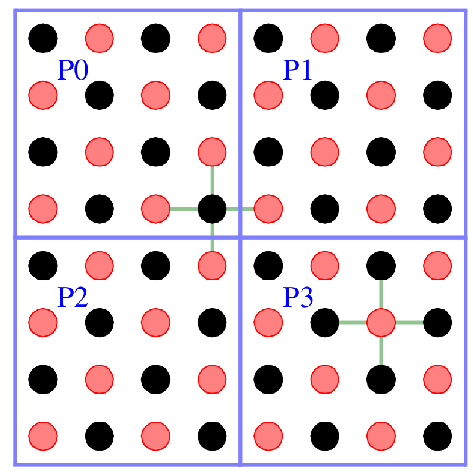
\includegraphics{redblack.pdf}
  \caption{The red-black grid divided into four subgrids. The image is from the exercise sheet}
\end{figure}

Once all iterations are complete, all the subgrids are merged and the solution is returned.

\section{Documentation}
%a) Presentation of the code
A point is updated by running the following function
\begin{lstlisting}[language=C++]
double f( double f, double l, double r, 
          double d, double u, double g, int N )
{ 
  double gam = 0.1;
  return (1-gam)*f + gam*0.25*(l+r+u+d - g/pow(N,2) );
}
\end{lstlisting}
The input variable \verb|f| corresponds to the current value at the point. Values \verb|l|, \verb|r|, \verb|u|, and \verb|d| correspond to the values on the left, right, up, and down respectively.
\verb|g| corresponds to $g_{i,j}$ and \verb|N| is the number of rows or columns $N$.

\subsection{Red Black function}
The program is made to run on 1, 2 or 4 cores.
The parallelization is implemented with MPI.
Initially I wanted the number of cores to be arbitrary but this turned out to be more difficult.
\begin{lstlisting}[language=C++]
void red_black( double** M, int N, int iters, int id, int ntasks )
{
  if ( !(ntasks==1 || ntasks==2 || ntasks==4 ) ) {
    throw invalid_argument("Number of processes should be 1, 2 or 4");
  }
\end{lstlisting}
\verb|M| is the grid represented as a two-dimensional array, \verb|iters| is the number of iterations, \verb|id| the index of the current subprocess, and \verb|ntasks| the total number of subprocesses.
The boundary values of \verb|M| should be initialized before calling \verb|red_black| function.

Next the boundaries for each subprocesses are set:
\begin{lstlisting}[language=C++]
  int x_min = 1;
  int y_min = 1;
  int x_max = N-1;
  int y_max = N-1;
  int id_lr, id_tb, id_top, id_bottom;

  // Setting boundaries for each
  // parallel process
  if (ntasks != 1) {
    if ( id%2 == 0 ) {
      x_max = x_max / 2;
      id_lr = id+1;
    } else {
      x_min = x_max / 2;
      id_lr = id-1;
    }
    if (ntasks == 4) {
      if ( id<2 ) {
        y_max = y_max / 2;
        id_bottom = id+2;
        id_tb = id+2;
      } else {
        y_min = y_max / 2;
        id_top = id-2;
        id_tb = id-2;
      }
    }
  }
\end{lstlisting}
If the number of the subprocesses is 2, the grid is divided into two rectangles.
For 4 subprocesses the grid is divided into four squares of the same size in a similar way as in Figure 1.

The main iteration loop performs the following steps
\begin{enumerate}
  \item
    Update the red sublattice
  \item
    Synchronize the values of the grid at the border of a subprocess with the corresponding neighbouring subprocess
  \item
    Update the black sublattice
  \item
    Synchronize again
\end{enumerate}

\begin{lstlisting}[language=C++]
  
  for ( int k=0; k<iters; k++ ) {
    // RED sublattice
    for ( int i=x_min; i<x_max ; i++ ) {
      for ( int j=i%2+y_min ; j<y_max; j+=2 ) {
        M[i][j] = f(M[i][j], M[i-1][j], M[i+1][j], M[i][j-1], M[i][j+1], g(i,j,N), N);
      }
    }
    // Sync
    if (ntasks != 1) {
      update_lr(M,N,id,x_min,x_max,id_lr);
      if (ntasks == 4) update_tb(M,N,id,x_min,x_max,y_min,y_max,id_tb);
    } 

    // BLACK sublattice
    for ( int i=x_min; i<x_max; i++ ) {
      for ( int j=(i+1)%2+y_min; j<y_max; j+=2 ) {
        M[i][j] = f(M[i][j], M[i-1][j], M[i+1][j], M[i][j-1], M[i][j+1], g(i,j,N), N);
      }
    }
    // Sync
    if (ntasks != 1) {
      update_lr(M,N,id,x_min,x_max,id_lr);
      if (ntasks == 4) update_tb(M,N,id,x_min,x_max,y_min,y_max,id_tb);
    } 
  }
\end{lstlisting}
The function for $g_{i,j}$ is hardcoded into the program.
If one wishes to run the code with different $g_{i,j}$, the function should be altered accordingly.

Once the iterations are performed, the values are merged into the array of subprocess 0.
If the number of subprocesses if 4, we first merge the bottom subsgrids with the corresponding top subgrids.
\begin{lstlisting}[language=C++]
  // MERGE THE RESULTS
  
  // For four subprocesses, first the top subgrid 
  // is merged with the corresponding bottom subgrid
  if (ntasks == 4) {
    if (id < 2) {
      int from_id = id+2;
      for (int j=y_max; j<N-1; j++) {
        for (int i=x_min; i<x_max; i++) {
          MPI_Recv(&M[i][j], 1, MPI_DOUBLE, from_id, 1, MPI_COMM_WORLD, MPI_STATUS_IGNORE);
        }
      }
    } else {
      int to_id = id-2;
      for (int j=y_min; j<y_max; j++) {
        for (int i=x_min; i<x_max; i++) {
          MPI_Send(&M[i][j], 1, MPI_DOUBLE, to_id, 1, MPI_COMM_WORLD);
        }
      }
    }
  }
\end{lstlisting}

After this, the process for 4 and 2 subprocess is the same:
Merge the left and right subgrids.
\begin{lstlisting}[language=C++]

  // Left and right subgrids merged
  if (ntasks != 1) {
    if (id == 0) {
      int from_id = 1;
      for (int i=x_max; i<N-1; i++) {
        MPI_Recv(M[i], N, MPI_DOUBLE, from_id, 1, MPI_COMM_WORLD, MPI_STATUS_IGNORE);
      }
    } else if (id == 1) {
      for (int i=x_min; i<x_max; i++) {
        MPI_Send(M[i], N, MPI_DOUBLE, 0, 1, MPI_COMM_WORLD);
      }
    }
  }
\end{lstlisting}

\subsection{Running the algorithm}
MPI is initialized in the \verb|main| function:
\begin{lstlisting}[language=C++]
int main(int argc, char *argv[])
{
  int rc = MPI_Init(&argc, &argv);
  if (rc!=MPI_SUCCESS) {
    cout << "MPI_Init failed!" << endl;
    return 1;
  }

  int ntasks;
  MPI_Comm_size(MPI_COMM_WORLD, &ntasks);

  int id;
  MPI_Comm_rank(MPI_COMM_WORLD, &id);

\end{lstlisting}
After this we initialize the grid of size $N\times N$
\begin{lstlisting}[language=C++]
  int N = 30;
  double** M = new double*[N];
  for (int i = 0; i < N; i++) {
    // Declare a memory block of size n
    M[i] = new double[N];
  }
  for (int j = 0; j < N; j++) {
    for (int i = 0; i < N; i++) {
      M[j][i] = 0;
    }
  }

  for (int i=0; i<N; i++) {
    M[i][0] = boundary(i,0,N);
    M[i][N-1] = boundary(i,N-1,N);
    M[0][i] = boundary(0,i,N);
    M[N-1][i] = boundary(N-1,i,N);
  }
\end{lstlisting}

We may then print the matrix before and after running the algorithm.
\begin{lstlisting}[language=C++]

  cout << fixed << setprecision(2);
  for (int i=0; i<N; i++) {
    for (int j=0; j<N; j++) {
      cout << M[i][j] << " ";
    }
    cout << endl;
  }

  red_black( M, N, 100000, id, ntasks );

  this_thread::sleep_for(chrono::seconds(id));
  cout << endl;
  cout << id << endl;
  for (int i=0; i<N; i++) {
    for (int j=0; j<N; j++) {
      cout << R[i][j] << " ";
    }
    cout << endl;
  }

\end{lstlisting}

If one wishes to tun the algorithm for different $g_{i,j}$ and boundary conditions, the corresponding functions should be altered accordingly.

%\\
%b) Instructions for using the code
\section{Benchmarking}
%a) Details of the computing environment\\
%b) What did you measure, how did you measure, analysis
As the Poisson's equation is often encountered in the context of electrodynamics, I thought it would be interesting to see how the program performs when considering a single "charge" and the potential distribution it generates.
In electrodynamics the Poisson's equation takes the form
\begin{align*}
  \nabla^2 V &= -\frac{\rho}{\epsilon_0},
\end{align*}
where $V$ is (3-dimensional) potential, $\rho$ is the charge density and $\epsilon_0$ is the vacuum permittivity.

Since the program solves only two dimensional Poisson's equation, the common expression for the potential
\begin{align*}
  V(x,y,z) &= \frac{1}{4\pi \epsilon_0} \frac{1}{\sqrt{(x-x_0)^2+(y-y_0)^2+(z-z_0)^2}}
\end{align*}
cannot be used.
Instead, a new expression has to be derived.
In case of a unit charge, the charge density becomes $\rho(x,y)=\delta((x-x_0)^2+(y-y_0)^2)$.
Now solving the Poisson's equation corresponds to finding the Green's function
\begin{align*}
  1 &= \iint  \delta((x-x_0)^2+(y-y_0)^2)\dd x\dd y \\
  &= -\epsilon_0 \iint \left(
  \frac{\partial^2}{\partial x^2}G(x,y)
  +\frac{\partial^2}{\partial y^2}G(x,y)
  \right)\dd x\dd y 
\end{align*}
This equation is satisfied with $G(x,y) = -\frac{1}{2\pi \epsilon_0}\ln\sqrt{(x-x_0)^2+(y-y_0)^2}$, although I'm not going to show it here.
%\begin{align*}
%  &\frac{1}{2\pi}\iint \left(
%  \frac{\partial^2}{\partial x^2}
%  +\frac{\partial^2}{\partial y^2}
%  \right)\ln\sqrt{(x-x_0)^2+(y-y_0)^2} \dd x\dd y \\
%  &=\frac{1}{4\pi}\iint \left(
%  \frac{\partial}{\partial x}
%\frac{2(x-x_0)}{(x-x_0)^2+(y-y_0)^2} 
%  +\frac{\partial}{\partial y}
%\frac{2(y-y_0)}{(x-x_0)^2+(y-y_0)^2} 
%\right)
%\dd x\dd y \\
%  &=\frac{1}{2\pi}\iint \left(
%\frac{2}{(x-x_0)^2+(y-y_0)^2} 
%-
%\frac{2(x-x_0)^2+2(y-y_0)^2}{((x-x_0)^2+(y-y_0)^2)^2} 
%\right)
%\dd x\dd y \\
%  &=\frac{1}{\pi}\iint \left(
%\frac{1}{r^2} 
%-
%\frac{r\cos\theta+r\sin\theta}{r^4} 
%\right)
%r\dd r \dd \theta\\
%  &=\frac{1}{\pi}\int \left(
%\frac{1}{r} 
%+
%\frac{\cos\theta-\sin\theta}{r^2} 
%\right)
%\dd r \\
%  \frac{1}{2 \pi}\int \ln|\vb{r}-\vb{r}_0|
%  \dd^2 \vb{r}
%  &=
%  \frac{1}{2 \pi}\int \ln|{r}^2+r_0^2-r{r}_0\cos \theta|\dd r\dd\theta
%\end{align*}

I'm going to make the substitution $2\pi \delta=g(x,y)$.
The Poisson's equation takes the form
\begin{align*}
  \ln\sqrt{(x-x_0)^2+(y-y_0)^2} &= g(x,y) = 2 \pi\delta((x-x_0)^2+(y-y_0)^2) 
\end{align*}
In discretized coordinates this becomes
\begin{align*}
  \ln\sqrt{(i-i_0)^2+(j-j_0)^2} &= 2 \pi N^2.
\end{align*}

As the expression for $g_{i,j}$ and $f_{i,j}$ is defined, we can now run the program to see whether it will compute similar solution for $f$.
In the code the values for $i_0$ and $j_0$ are set as $N/4$ and $N\cdot3/4$ respectively.

The program converges to the correct values around the point well, but the value at the point itself is quite off.

I didn't manage to do proper benchmarking as I was running out of time.

\section{Conclusions}
%a) Summary\\
The algorithm manages to converge to a numerical solution for the 2D Poisson's equation on a square with the exception of the "source" point.
The parallelization gives a noticeable improvement improvement over a single core computation, although proper benchmarking on the results is missing.

%b) possible improvements

The program would have benefited from GUI but I was running out of time.
Or even just saving an image file for a computed solution.
Some refactoring would also be appropriate.
The current way of having hardcoded function for $g_{i,j}$ is not ideal. 
It could be perhaps better to have a function as an additional parameter for \verb|red_black| function.
The whole algorithm should also be moved to a separate file.
Also, I think it would be better to have some error value instead of a discrete number of iterations.

The program could be expanded to run on more cores.
In that case it would also be beneficial to make the code run on an arbitrary number of cores rather than having some specific set of options (as in this case 1, 2 and 4).

There are minor adjustments which could be made to avoid some unnecessary steps.
For example on the "Sync" step, a subprocess sends and receives all values at the boundary even though only half of them are used before encountering the next sync step.
I don't believe this has any significant effect on the runtime of the algorithm, but could be done in order to get as good performance as possible.
I would also imagine that MPI probably has some methods for merging the different subgrids into one.
My method here seems to be unnecessarily sloppy.

My biggest regret here is that I started to work on this too late despite the generous deadline.

\begin{thebibliography}{9}
\bibitem{NumRec}
William H. Press, Saul A. Teukolsky, William T. Vetterling, Brian P- Flannery, Numerical Recipes in C, Second Edition (1992), Cambridge University Press
\end{thebibliography}
\end{document}

